\documentclass[letterpaper,12pt]{article}
%\usepackage{harvard}
%\usepackage{subfigure}
%\usepackage[active]{srcltx}
\usepackage{graphicx}
\usepackage{pdflscape}
\usepackage{amsmath}
\usepackage{amsthm}
\usepackage{lscape}
\usepackage{enumerate}
\usepackage{float}
\usepackage{grffile}
\usepackage{relsize}
\usepackage{tablefootnote}
\usepackage{footnote}
\usepackage{sectsty}
\usepackage{xcolor}
\usepackage{caption}
\usepackage{color}
\usepackage{natbib}
\usepackage{multirow}
\usepackage{bbm}
\usepackage[T1]{fontenc}
\usepackage[multiple]{footmisc}
\usepackage{appendix}
\usepackage{times}
\usepackage{relsize}
\usepackage{caption}
\usepackage{newtxtext,newtxmath}
\usepackage{enumitem}


%%%%%%%%%%%%%%%%%%%%%%%%%%%%%%%%%%%%%%%%%%%%%%%%%%%%%%%%%%%%
%%%   Title Page Information
%%%%%%%%%%%%%%%%%%%%%%%%%%%%%%%%%%%%%%%%%%%%%%%%%%%%%%%%%%%%
\title{ECON311: Assignment I-Solutions}
\author{Leandro Freylejer}
\date{}
%%%%%%%%%%%%%%%%%%%%%%%%%%%%%%%%%%%%%%%%%%%%%%%%%%%%%%%%%%%%
%%%   Double and Single Space Commands
%%%%%%%%%%%%%%%%%%%%%%%%%%%%%%%%%%%%%%%%%%%%%%%%%%%%%%%%%%%%
\newlength{\defbaselineskip}
\setlength{\defbaselineskip}{\baselineskip}
\newcommand{\setlinespacing}[1]{\setlength{\baselineskip}{#1 \defbaselineskip}}
\newcommand{\doublespacing}{\setlength{\baselineskip}{1.3 \defbaselineskip}}
\newcommand{\singlespacing}{\setlength{\baselineskip}{1\defbaselineskip}}
\renewcommand{\thesubsection}{\arabic{subsection}}
\newtheoremstyle{dotlessS}{}{}{\itshape}{}{\color{dg}\bfseries}{}{ }{}
\theoremstyle{dotlessS}
\newtheorem{theorem}{Theorem}
\newtheorem{lemma}{Lemma}
\newtheorem{proposition}{Proposition}
\newtheorem{assumption}[theorem]{Assumption}
\newtheorem{corollary}{Corollary}
\newtheorem{definition}{Definition}
\newenvironment{example}[1][Example]{\begin{trivlist}
\item[\hskip \labelsep {\bfseries #1}]}{\end{trivlist}}
\newenvironment{remark}[1][Remark]{\begin{trivlist}
\item[\hskip \labelsep {\bfseries #1}]}{\end{trivlist}}

\newcommand\Pitem{%
  \addtocounter{enumi}{-1}%
  \renewcommand\theenumi{\arabic{\enumi}'}%
  \item%
  \renewcommand\theenumi{\arabic{enumi}}%
}

%%%%%%%%%%%%%%%%%%%%%%%%%%%%%%%%%%%%%%%%%%%%%%%%%%%%%%%%%%%%
%%%   Set Margins Here
%%%%%%%%%%%%%%%%%%%%%%%%%%%%%%%%%%%%%%%%%%%%%%%%%%%%%%%%%
\textwidth=6.5in
\textheight=9in
\oddsidemargin=0.10in
\evensidemargin=0.10in
\topmargin=-0.5in
%\parskip=3pt

%%%%%%%%%%%%%%%%%%%%%%%%%%%%%%%%%%%%%%%%%%%%%%%%%%%%%%%%%%%%%
%%%   Actual Document Begins Here
%%%%%%%%%%%%%%%%%%%%%%%%%%%%%%%%%%%%%%%%%%%%%%%%%%%%%%%%%%%%%
\begin{document}
\pagenumbering{arabic}
\maketitle
\vspace{-.6in}
\section*{Question I [10 points]}
Complete the following table:
\begin{table}[H]
\begin{minipage}[h]{1\textwidth}
\centering
\resizebox{18cm}{!}{%
\begin{tabular}{|l|l|l|l|l|l|l|l|l|}

\hline
			&     &   	     &            &        &          &                                     &                              &                   \\[1.2ex]
Year            &Price of     &Quantity of     &Price of               &Quantity of       &RGDP Chained Weighted           &$\%\Delta RGDP_{F}$ & $GDP^{deflator}$ & Inflation \\
			&Burgers    &Burgers  	     &Magazines            &Magazines        &Prices  benchmark to 2014         &                                     &                              &  Rate                  \\[2.4ex]
\hline
			&     &   	     &            &        &          &                                     &                              &                   \\[1.2ex]
2013	       &$\$4.00$ &100                 &$\$2.00$               &180				& $\$949.91$       &                                & 0.8                             &                   \\[2.4ex]
2014	       &$\$5.00$	&120		     &$\$2.50$	          &200      		      & $\$1100$          &       $15.79\%$         &  1                            &$25\%$                   \\[2.4ex]
2015             &$\$6.00$	&150		     &$\$3.50$                &200		      & $\$1245.2$       &       $13.16\%$         &  1.28                        &$28\%$                   \\[2.4ex]
\hline
\end{tabular}}
\end{minipage} 
\end{table}
\textbf{Answer:}
\begin{enumerate}
\item Laspeyres:
\begin{eqnarray*}
\begin{array}{l}
RGDP_{\$2013}^{2013}=\$4.00 \: \: 100+\$2.00 \: \: 180=\$760  \\[1.2ex]
RGDP_{\$2013}^{2014}=\$4.00 \: \: 120+\$2.00 \: \: 200=\$880  \\[1.2ex]
\% \Delta RGDP_L^{2014}=\frac{880-760}{760} \: \: 100=15.79\%   \\[1.4ex]
RGDP_{\$2014}^{2014}=\$5.00 \: \: 120+\$2.50 \: \: 200=\$1100  \\[1.2ex]
RGDP_{\$2014}^{2015}=\$5.00 \: \: 150+\$2.50 \: \: 200=\$1250  \\[1.2ex]
\% \Delta RGDP_L^{2015}=\frac{1250-1100}{1100} \: \: 100=13.64\%  
\end{array}
\end{eqnarray*}
\item Paasche:
\begin{eqnarray*}
\begin{array}{l}
RGDP_{\$2014}^{2013}=\$5.00 \: \: 100+\$2.50 \: \: 180=\$950 \\[1.2ex]
RGDP_{\$2014}^{2014}=\$5.00 \: \: 120+\$2.50 \: \: 200=\$1100  \\[1.2ex]
\% \Delta RGDP_P^{2014}=\frac{1100-950}{950} \: \: 100=15.79\%   \\[1.4ex]
RGDP_{\$2015}^{2014}=\$6.00 \: \: 120+\$3.50 \: \: 200=\$1420  \\[1.2ex]
RGDP_{\$2015}^{2015}=\$6.00 \: \: 150+\$3.50 \: \: 200=\$1600  \\[1.2ex]
\% \Delta RGDP_L^{2015}=\frac{1600-1420}{1420} \: \: 100=12.68\%  
\end{array}
\end{eqnarray*}
\item Fisher
\begin{eqnarray*}
\begin{array}{l}
\% \Delta RGDP_F^{2014}=\frac{\% \Delta RGDP_L^{2014}+\% \Delta RGDP_P^{2014}}{2}=15.79 \\[1.4ex]
\% \Delta RGDP_F^{2015}=\frac{\% \Delta RGDP_L^{2015}+\% \Delta RGDP_P^{2015}}{2}=13.16
\end{array}
\end{eqnarray*}
\item Nominal GDP
\begin{eqnarray*}
\begin{array}{l}
NGDP_{2013}=\$4.00 \: \: 100+\$2.00 \: \: 180=\$760  \\[1.2ex]
NGDP_{2014}=\$5.00 \: \: 120+\$2.50 \: \: 200=\$1100  \\[1.2ex]
NGDP_{2015}=\$6.00 \: \: 150+\$3.50 \: \: 200=\$1600  \\[1.2ex]
\end{array}
\end{eqnarray*}
\item RGDP Chained Weighted Prices benchmark to 2014
\begin{eqnarray*}
\begin{array}{l}
RGDP^{2013}=\frac{NGDP^{2014}}{\left(1+\frac{\% \Delta RGDP_F^{2014}}{100}\right)}=\$949.91  \\[4ex]
RGDP^{2014}=NGDP^{2014}=\$1100  \\[1.2ex]
RGDP^{2015}=NGDP^{2014} \: \: \left(1+\frac{\% \Delta RGDP_F^{2014}}{100} \right)=\$1245.2
\end{array}
\end{eqnarray*}
\item GDP Deflator
\begin{eqnarray*}
\begin{array}{l}
GDP^{def}_{2013}=\frac{NGDP_{2013}}{RGDP^{2013}}=0.8 \\[1.2ex]
GDP^{def}_{2014}=\frac{NGDP_{2014}}{RGDP^{2014}}=1 \\[1.2ex]
GDP^{def}_{2015}=\frac{NGDP_{2015}}{RGDP^{2015}}=1.28 \\[1.2ex]
\end{array}
\end{eqnarray*}
\item Inflation
\begin{eqnarray*}
\begin{array}{l}
INF^{2014}=\frac{GDP^{def}_{2014}-GDP^{def}_{2013}}{GDP^{def}_{2013}} \: \: 100 =25\%  \\[1.2ex]
INF^{2015}=\frac{GDP^{def}_{2015}-GDP^{def}_{2014}}{GDP^{def}_{2014}} \: \: 100 =28\% 
\end{array}
\end{eqnarray*}
\end{enumerate}

\section*{Question II}
For this question you will need to download four data series. You can find all data at the World Bank Development Indicators website (https://databank.worldbank.org/data/source/world-development-indicators). The series needed to answer this question are: i. ``GDP per capita (constant 2015 $US\$$)'', ii. ``GDP per capita, PPP (constant 2021 international $\$$)''. You need to obtain these data series for both Canada and Chile from 1993 to 2017. To analyze the data you are free to use any software you would like. I recommend that you use Microsoft Excel because you can directly download the series in Excel format. If you do not have Excel in your personal computer, you can access it through the university's server.
\begin{enumerate}[label=\alph*]
\item (10 points) Plot both GDP per capita (constant 2015 $US\$$) series on the same graph with time on the horizontal axis and GDP per capita on the vertical axis. On a different graph, plot both GDP per capita, PPP (constant 2021 international $\$$) series with time on the horizontal axis and GDP per capita on the vertical axis. Which series are better in understanding differences in well-being across countries? Explain.\\
\\
\\
\textbf{Answer:}
\begin{figure}[h!]
\centering
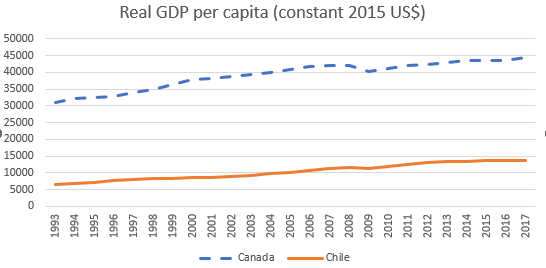
\includegraphics[scale=.85]{RGDP_Constant_Prices}
\end{figure}
\begin{figure}[h!]
\centering
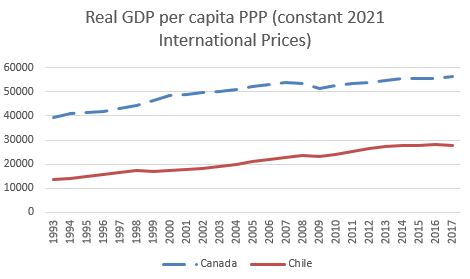
\includegraphics[scale=.95]{RGDP_PPP_Prices}
\end{figure}
\\
\\
The series with constant prices is likely to overestimate the differences in real GDP per capita between Canada and Chile. The reason for this is that prices tend to be lower in developing countries. The Price Purchasing Power (PPP) series adjusts for this by controlling for price differences, which makes the real GDP per capita PPP a better measure of differences in well-being across countries. 
\item (10 points) Assume that in any given year, the GDP of a country is given by the production function studied in class ($Y=\overline{A}(K)^{\frac{1}{3}}(L)^{\frac{2}{3}}$). Also, as in class, assume that there are no differences in $\overline{A}$ across countries. Using the GDP per capita, PPP, calculate the annual differences in capital per capita for each year. Plot the amount of capital per capita in Canada relative to the amount of capital per capita in Chile for each year. Given our discussion in class, does this measure represent the actual differences in capital per capita? Explain.     \\
\\
\\
\textbf{Answer:}
\begin{figure}[h!]
\centering
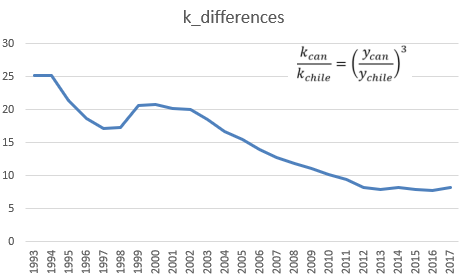
\includegraphics[scale=.85]{k_differences}
\end{figure}
\\
\\
This measure does not represent the actual differences in capital per capita because we are assuming that both countries have the same level of TFP ($\overline{A}$). It is likely that total factor productivity is larger in Canada than in Chile, therefore, the previous measure  overestimates the differences in capital per capita across these two countries
\item (10 points) Using  GDP per capita, PPP (constant 2021 international $\$$) calculate the average annual growth rates for the Chilean and Canadian economies for the entire period. Assume that the Chilean economy keeps growing at a constant rate equal to the average annual rate for the 1993-2017 period. How many more years would it take for the GDP per capita in Chile to reach the level of GDP per capita in Canada in 2017? \\
\\
\textbf{Answer:}
\begin{eqnarray*}
\begin{array}{c}
\overline{g}_{CAN}=\left(\frac{56522.015}{39559.269}\right)^{\frac{1}{24}}-1=0.015 \\[2ex]
\overline{g}_{Chile}=\left(\frac{27929.476}{13479.629}\right)^{\frac{1}{24}}-1=0.0308 \\[2ex]
T=\frac{ln\left(\frac{56522.015}{27929.476}\right)}{0.0308}\approx 22.8879
\end{array}
\end{eqnarray*}
\end{enumerate}  

\section*{Question III}
Suppose that total GDP in a country at a given year is given by the following production function:
\begin{eqnarray*}
Y=\overline{A}(K)^{\frac{1}{3}}(\beta L)^{\frac{2}{3}} 
\end{eqnarray*}
where $\beta$ represents labour productivity and all other variables are the same as in class. The introduction of $\beta$ expands the production model by allowing production to also depend on the human capital or productivity of the labour force.  Assume that there are two countries with the same number of workers ($\overline{L}$) and total factor productivity ($\overline{A}$) but with different levels of labour productivity ($\beta$). In particular, we are going to assume that the labour force in one country is twice as productive as the the labour force in the other country.
\begin{enumerate}[label=\alph*]
\item (10 points) Calculate differences in GDP as a function of differences in the amount of physical capital, $K$, across countries. In a graph with GDP differences on the vertical axis and differences in physical capital on the horizontal axis, plot this function. In the same graph show what happens when labour productivity differences increase.\\
\\
\textbf{Answer:}\\
Let country $1$ have twice as much human capital as country 2 (i.e. $\beta_1=2 \: \: \beta_2$), then:
\begin{figure}[h!]
\centering
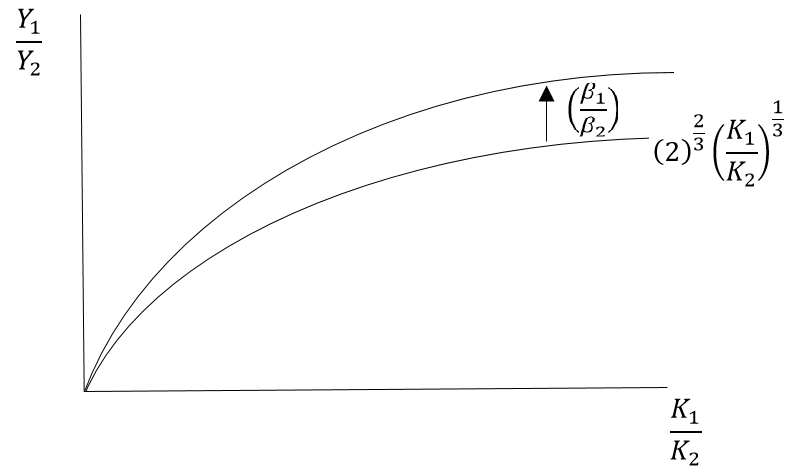
\includegraphics[scale=.54]{labour_productivity}
\end{figure}
\\
\\
\item (10 points) Assume that, in both countries, $\overline{L}$ grows at a constant rate $g_L$, $\overline{K}$ grows at a constant rate $g_K$, $\overline{A}$ grows at a constant rate $g_A$ and $\beta$ grows at a constant rate $g_{\beta}$. Calculate the constant rate of growth of GDP, $g_Y$, and GDP per capita, $g_y$.   \\
\\
\textbf{Answer:}\\
Using the arithmetic laws of growth rates, we obtain:
\begin{eqnarray*}
\begin{array}{l}
g_Y=g_A+\frac{1}{3}g_K+\frac{2}{3}g_L+ \frac{2}{3}g_{\beta} \\[2ex]
 g_y=g_A+\frac{1}{3}(g_K-g_L)+ \frac{2}{3}g_{\beta} 
\end{array}
\end{eqnarray*}
\end{enumerate}

\section*{Question IV [15 points]}
Consider a one-time change in immigration policy that immediately and permanently increases the level of the labour force in an economy. Suppose it rises permanently from $\overline{L}$ to $\overline{L}'$. Assuming the economy starts in its initial steady state, use the Solow model to explain what happens to the economy over time (transition dynamics) and in the long run (steady state). In particular, discuss what happens to the levels of capital, capital per worker, GDP and GDP per worker both at the new steady state as well as during the transition to the new steady state. You are \textbf{not} required to discuss how growth rates change over time (this is tricky). To answer this question use both the Solow diagram with total output, and diagrams with time on the horizontal axis and each of these variables on the vertical axis.  \\
\\
\textbf{Answer:}\\
At the steady-state equilibrium:
\begin{eqnarray*}
\begin{array}{lll}
K^*=\overline{L}\left(\frac{\overline{s}\overline{A}}{\overline{d}}\right)^{\frac{2}{3}} & , &k^*=\left(\frac{\overline{s}\overline{A}}{\overline{d}}\right)^{\frac{2}{3}}  \\[2ex]
Y^*=\overline{A}\left(K^*\right)^{\frac{1}{3}} \left(\overline{L}\right)^{\frac{2}{3}} &, & y^*=\overline{A}\left(k^*\right)^{\frac{1}{3}}
\end{array}
\end{eqnarray*}
So, at the steady-state equilibrium after the shock to labour supply: $K^*\uparrow$, $Y^*\uparrow$, $k^*=$, $y^*=$
\begin{figure}[h!]
\centering
\caption*{Solow Model}
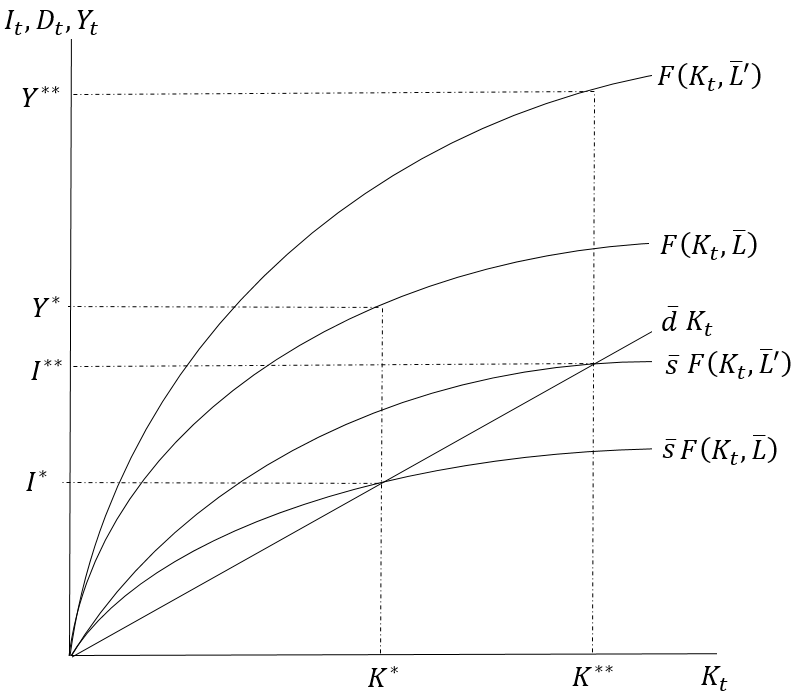
\includegraphics[scale=.54]{increase_labour_force}
\end{figure}
\begin{figure}[h!]
\centering
\caption*{Transition Dynamics I}
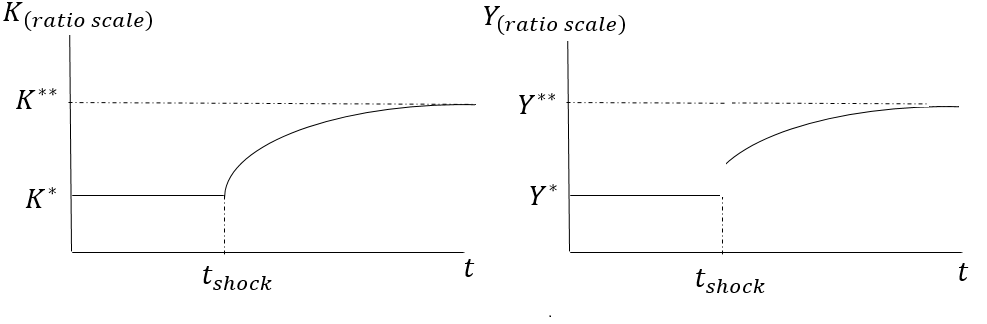
\includegraphics[scale=.54]{transition_dynamics}
\end{figure}
\begin{figure}[h!]
\centering
\caption*{Transition Dynamics II}
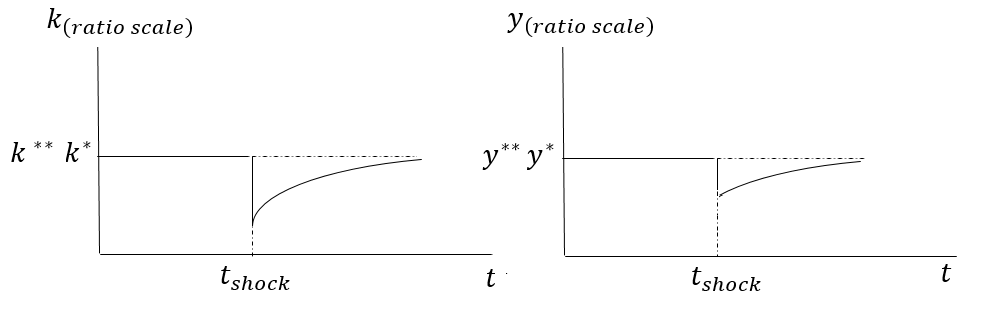
\includegraphics[scale=.54]{transition_dynamics_per_capita}
\end{figure}\\
\\


\section*{Question V}
Consider a Solow model where the production function no longer exhibits diminishing returns to capital accumulation. Assume that the production function is now $Y_t=\overline{A}K_t$. The rest of the model is unchanged.
\begin{enumerate}[label=\alph*]
\item (5 points) Draw the Solow diagram in this case.\\
\\
\textbf{Answer:}\\
The Law of Motion is: $\Delta K_{t+1}=(\overline{s}\overline{A}-\overline{d})K_t$. I am going to assume that: $\overline{s}\overline{A}>\overline{d}$
\begin{figure}[h!]
\centering
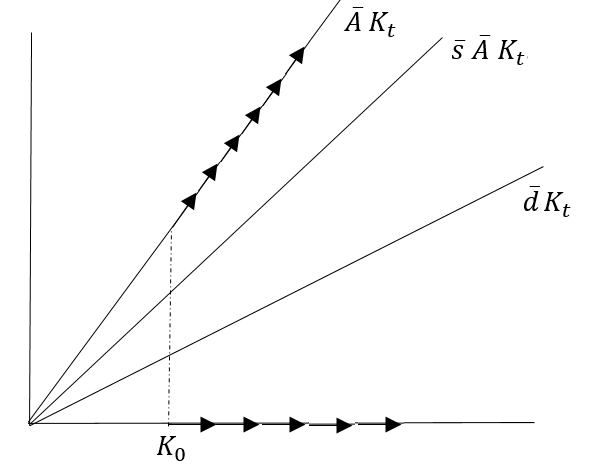
\includegraphics[scale=.4]{constant_growth_solow}
\end{figure}\\
\\
\\
\item (5 points) Suppose the economy begins with capital $\overline{K}_0$, and show how the economy evolves over time in the Solow model.\\
\\
\textbf{Answer:}\\
Refer to the previous figure. Net investment is always postive, so $\Delta K_{t+1}>0$ for all $t=1,..$, so $K_t$ and $Y_t$ keep growing forever.
\item (5 points) What happens to the growth rate of per capita GDP over time?\\
\\
\textbf{Answer:}\\
We can rewrite the production function in per capita terms: $y_t=\overline{A}\frac{K_t}{\overline{L}}$. Using the arithmetic laws of growth:
\begin{eqnarray*}
\begin{array}{lll}
gy=g_A+g_K+g_L &\Rightarrow& gy=g_K=\frac{\Delta K_{t+1}}{K_t}=(\overline{s}\overline{A}-\overline{d})>0
\end{array}
\end{eqnarray*}

\end{enumerate}




\end{document}






